% --- ARCHIVO: Cap3_analisis_incidente/analisis_incidente.tex ---
\chapter{Anatomía del incidente: cronología del colapso (Fases 0 a 3)}
\label{cap:analisis_incidente}

\section{Fase 0: inestabilidad de tensiones y efecto del mallado}
\label{sec:fase_0_inestabilidad}

\lettrine[lines=3, lhang=0.1]{E}{l} escrutinio forense de la cronología demuestra que el cero de tensión no fue un evento instantáneo sino la culminación de una degradación progresiva de la estabilidad estática y dinámica de la red. Durante la Fase~0, los analizadores registraron una elevada volatilidad en l... escrutinio forense de la cronología demuestra que el cero de tensión no fue
un evento instantáneo sino la culminación de una degradación progresiva de la
estabilidad estática y dinámica de la red. Durante la Fase~0, los analizadores
registraron una elevada volatilidad en los perfiles de tensión ($V$) sobre una
topología extremadamente débil: ante la baja demanda, el 35,8~\% de la red de
400~kV en la zona sur y el 34,3~\% en la zona centro permanecían
desconectadas, configurando un escenario de alta \textit{impedancia de
transferencia}\textsuperscript{\ref{anexo:impedancia}} \cite{icai2025}.

Sobre esta red debilitada, la dinámica del sistema se manifestó en forma de
oscilaciones electromecánicas con dos modos diferenciados. A las
12:03:00~CEST se registró una primera \textit{oscilación forzada}\textsuperscript{\ref{anexo:oscilaciones}} de
0,6~Hz de carácter local,
que tardó 4 minutos y 42 segundos en amortiguarse. A las 12:19:00~CEST
emergió un segundo \textit{modo inter-área} de 0,2~Hz (Este-Centro-Oeste),
por el que la península ibérica comenzó a oscilar en contrafase respecto al
resto del continente, tensando la interconexión pirenaica \cite{entsoe2025}.
Durante ambos transitorios, el \textit{ratio de amortiguamiento}\textsuperscript{\ref{anexo:amortiguamiento}} se desplomó a valores
cercanos al 1~\%, vulnerando el umbral mínimo del 5~\% exigido por el
P.O.~13.1. Este comportamiento no era inédito: la operación prolongada en
régimen de ``red ligera'' había producido episodios análogos los días 16,
22 y 24 de abril, tratados entonces como incidencias aisladas en lugar de
síntomas de una degradación sistémica \cite{icai2025}.

\vspace{0.6cm}
\begin{figure}[H]
    \centering
    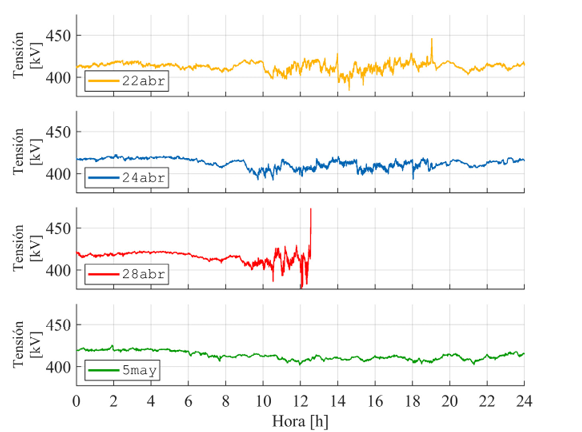
\includegraphics[width=0.75\textwidth]{figuras/nunez_balboa_precursores.png}
    \vspace{0.2cm}
    \caption[Tensiones registradas en Núñez de Balboa 400 kV (22, 24 y 28 de abril).]{%
    Tensiones registradas en la subestación de Núñez de Balboa, en la red
    de transporte de 400~kV, durante los eventos precursores y el día del
    incidente. Fuente: Informe pericial IIT-ICAI}
    \label{fig:precursores_nunez}
\end{figure}
\vspace{0.6cm}

La figura~\ref{fig:precursores_nunez} muestra los registros de tensión en
Núñez de Balboa durante los días 22, 24 y 28 de abril. La sucesión de
picos de sobretensión observada por el informe ICAI es interpretada por
dicho informe como indicio del estrechamiento progresivo de los márgenes
de control de potencia reactiva en la red de transporte.

Para contener estas oscilaciones, los operadores ejecutaron una maniobra
de mallado (\textit{meshing}): entre las 12:03 y las 12:30~CEST, REE
reconectó 11 líneas de 400~kV que permanecían abiertas por la baja
demanda. La maniobra logró su objetivo inmediato ---reducir la impedancia
y frenar el ``latigazo'' de las oscilaciones--- pero introdujo, según el
informe pericial del IIT-ICAI, un efecto secundario relevante en relación
con el incidente posterior: por el \textit{Efecto Ferranti}\textsuperscript{\ref{anexo:ferranti}}, las líneas
reconectadas en vacío inyectaron de forma abrupta una cantidad
significativa de potencia reactiva capacitiva en una red que ya carecía de
margen de absorción. La cuantificación exacta de esta inyección
constituye uno de los ejes centrales de la disputa técnica entre los
informes: el informe pericial de IIT-ICAI cifra el volumen en hasta
2,4~GVAr, mientras que el análisis independiente del Laboratorio Nacional
de Energías Renovables de EE.UU. (\textit{National Renewable Energy
Laboratory}, NREL) adopta una estimación más conservadora de 1.050~MVAr
\cite{icai2025, nrel2025}. Ambas cifras coinciden, no obstante, en
señalar que la inyección superó la capacidad de absorción residual del
sistema, estimada en ese momento en apenas 3,3~GVAr frente a los
5,8~GVAr habituales.

\vspace{0.6cm}
\begin{figure}[H]
    \centering
    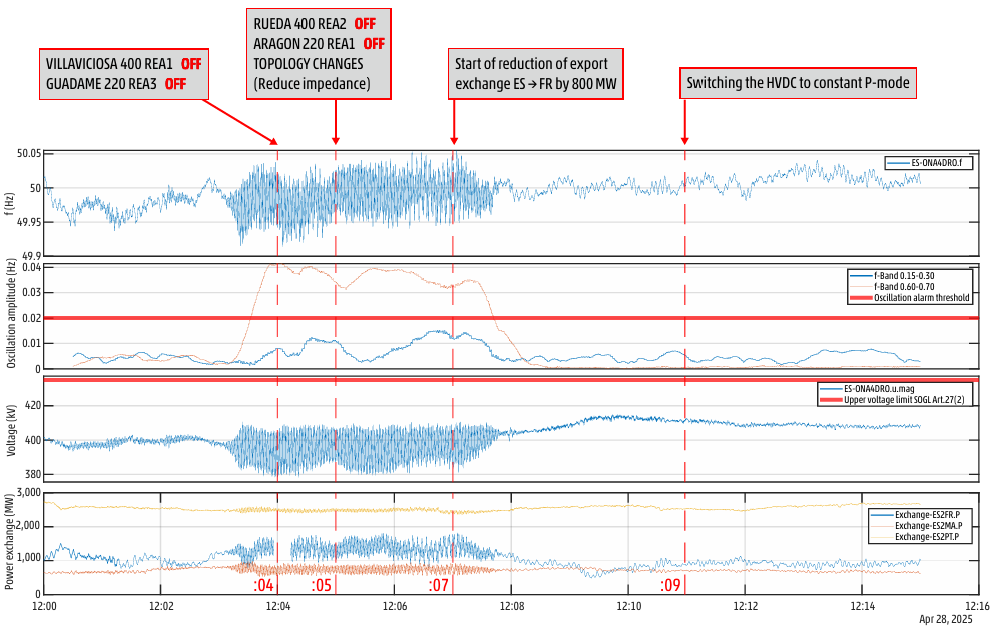
\includegraphics[width=0.95\textwidth]{figuras/wams_oscilaciones_carmona.png}
    \vspace{0.2cm}
    \caption[Registro WAMS de la primera oscilación de 0,6 Hz a las 12:03 CEST.]{%
    Registro de un \textit{Wide Area Monitoring System} (WAMS) que captura
    la oscilación electromecánica de 0,6~Hz medida en Carmona (Sevilla)
    a las 12:03~CEST. Fuente: Informe Factual ENTSO-E / REE}
    \label{fig:wams_carmona}
\end{figure}
\vspace{0.6cm}

La figura~\ref{fig:wams_carmona} muestra el registro WAMS de esta
oscilación. Los sistemas WAMS (\textit{Wide Area Monitoring Systems}) se
basan en redes de unidades de medida fasorial (PMU) sincronizadas por GPS,
que permiten observar simultáneamente la dinámica de la red en escalas
geográficas continentales con resolución de milisegundos. Su capacidad
para capturar modos electromecánicos de baja frecuencia los convierte en
la herramienta de referencia para el análisis forense de incidentes
sistémicos.

Esta inyección masiva saturó la capacidad de la red para absorber potencia
reactiva ($Q$), reduciendo el margen de seguridad de las \textit{curvas de
estabilidad de tensión Q-V}\textsuperscript{\ref{anexo:curvas_qv}}.
Las simulaciones periciales del IIT-ICAI estiman que, tras el mallado, la
distancia al punto de colapso en el nudo de Carmona~400~kV se contrajo de
un margen de 2.964~MW a 1.268~MW, una reducción próxima al 57~\% que
acercó al sistema a un estado de saturación capacitiva. Esta conclusión
técnica es el fundamento sobre el que el informe del IIT-ICAI ---elaborado
a petición de Endesa e Iberdrola--- construye su tesis de responsabilidad
operativa, en contraposición directa con la narrativa de incumplimiento
normativo sostenida por el Gobierno y REE, debate analizado en
profundidad en el capítulo~\ref{cap:analisis_informes}
(p.~\pageref{cap:analisis_informes}) \cite{icai2025}.

\clearpage
\section{Fase 1: fenómenos de oscilación y disparo raíz (12:32:57~CEST)}
\label{sec:fase_1_oscilacion_raiz}

La transición hacia el colapso sistémico se gestó durante la hora previa al apagón a través de una inestabilidad dinámica progresiva. A partir de las 12:00:00~CEST, el sistema ibérico experimentó oscilaciones electromecánicas que evidenciaron el coste operativo de funcionar con una inercia muy reducida. El primer evento disruptivo se registró a las 12:03:00~CEST: una oscilación de 0,6~Hz con una amplitud de 70~mHz que se sostuvo durante 4 minutos y 42 segundos antes de amortiguarse \cite{entsoe2025}.

La naturaleza de este transitorio es objeto de controversia entre los
informes. Red Eléctrica (REE) lo clasifica como una oscilación forzada
originada en el lazo de control de una planta fotovoltaica en la
provincia de Badajoz, mientras que los peritajes independientes del
IIT-ICAI argumentan que se trató de un modo natural inter-área
exacerbado por un \textit{ratio de amortiguamiento} sistémico de tan
solo el 1~\% ---muy por debajo del umbral mínimo del 5~\% exigido por
el P.O.~13.1---, cuyo origen vinculan a la ausencia de
\textit{Estabilizadores del Sistema de Potencia} (PSS,
\textit{Power System Stabilizers})\textsuperscript{\ref{anexo:pss}} en las centrales de
ciclo combinado de Andalucía, las cuales permanecían apagadas
\cite{icai2025}.

\vspace{0.6cm}
\begin{figure}[H]
    \centering
    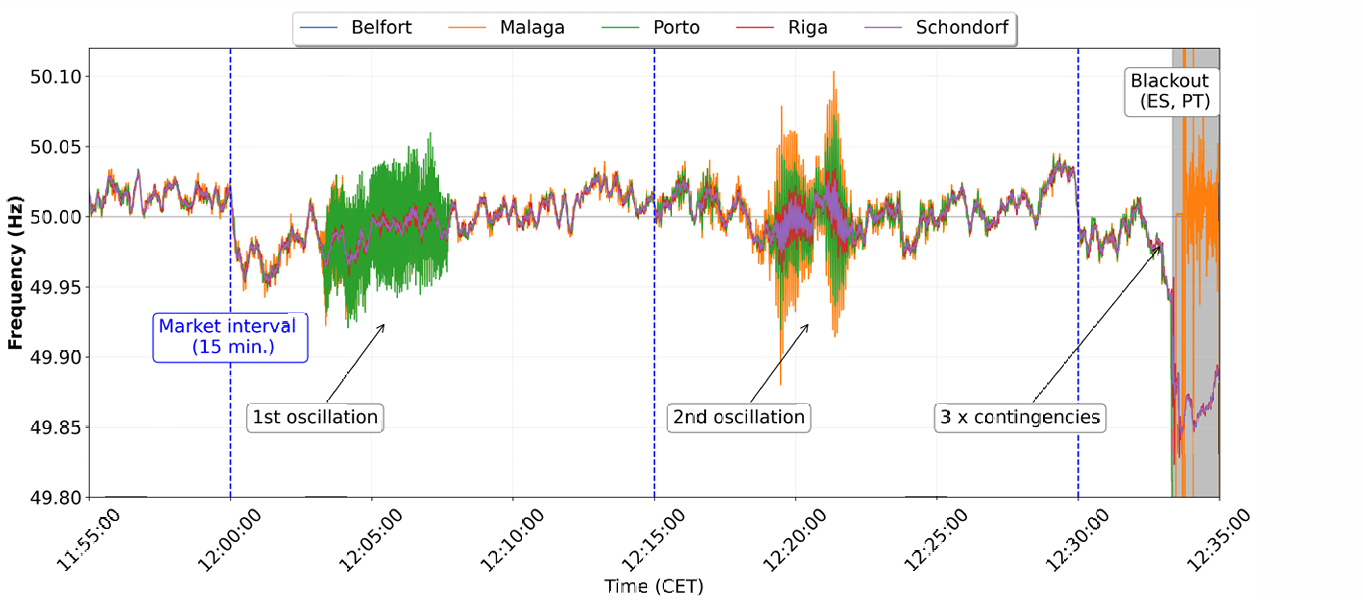
\includegraphics[width=0.9\textwidth]{figuras/timeline_frecuencia_nrel.png}
    \vspace{0.2cm}
    \caption[Visión general de la frecuencia del sistema durante la Fase 1.]{%
    Evolución de la frecuencia del sistema durante la Fase~1.
    Fuente: Análisis NREL}
    \label{fig:timeline_nrel}
\end{figure}
\vspace{0.6cm}

La figura~\ref{fig:timeline_nrel} reproduce el análisis de telemetría
externa elaborado por el NREL, en el que se aprecian las dos
oscilaciones electromecánicas y la pérdida progresiva de amortiguamiento
sistémico previa al colapso.

La inestabilidad se intensificó a las 12:19:00~CEST con la irrupción de
un segundo modo electromecánico, esta vez de 0,2~Hz y amplitud máxima
de 200~mHz. La telemetría fasorial (\textit{PMU}, \textit{Phasor
Measurement Units}) europea confirmó que este evento correspondía al
modo natural Este-Centro-Oeste del área síncrona continental: la
reducida masa rotatoria ibérica comenzó a oscilar en contrafase
respecto al centro de inercia europeo, tensando los enlaces de
interconexión pirenaicos. Es precisamente este mecanismo ---el
``efecto látigo'' descrito en la sección~\ref{sec:interconexiones}---
el que explica por qué una perturbación de escala moderada en el
centro del continente se amplificó hasta amplitudes notables en el
extremo ibérico \cite{nrel2025}.

\vspace{0.6cm}
\begin{figure}[H]
    \centering
    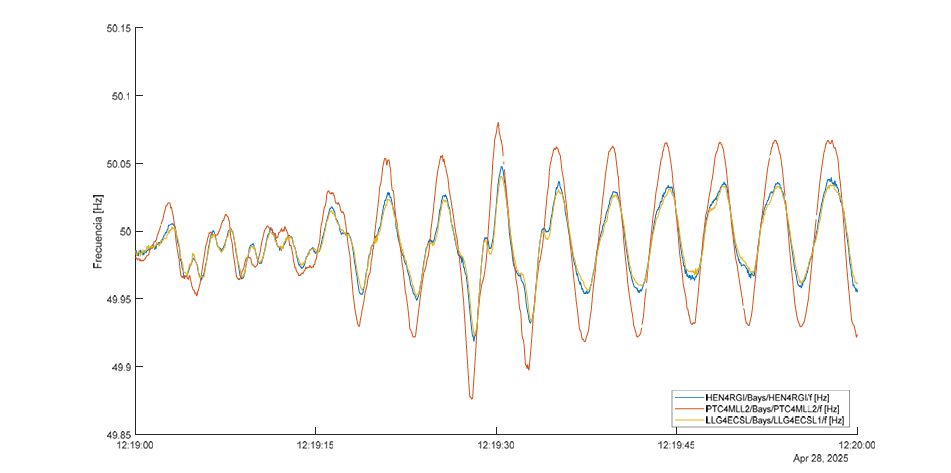
\includegraphics[width=0.9\textwidth]{figuras/oscilacion_hernani_icai.png}
    \vspace{0.2cm}
    \caption[Registro detallado de la segunda oscilación electromecánica a las 12:19 CEST.]{%
    Registro detallado de la oscilación electromecánica de 0,2~Hz a las
    12:19~CEST medida en la subestación de Hernani (Guipúzcoa).
    Fuente: Informe preliminar IIT-ICAI}
    \label{fig:oscilacion_hernani}
\end{figure}
\vspace{0.6cm}

Las divergencias de fase observadas en la figura~\ref{fig:oscilacion_hernani}
confirman, según el informe del IIT-ICAI, que el bloque ibérico oscilaba
en contrafase respecto al sistema síncrono continental europeo durante
los minutos previos al colapso.

Para amortiguar estas oscilaciones, el operador del sistema ejecutó dos
maniobras de urgencia: el mallado de la red de 400~kV ---detallado en
la sección~\ref{sec:fase_0_inestabilidad}--- y la fijación del enlace
HVDC con Francia en modo de potencia constante (1.000~MW de
exportación). Ambas decisiones lograron estabilizar la frecuencia,
pero, según el informe del IIT-ICAI, a un coste dinámico relevante
para la estabilidad de tensión: las maniobras saturaron la red de
potencia reactiva capacitiva, elevaron los perfiles de tensión y, en
opinión del peritaje, redujeron de forma sustancial los márgenes de
las \textit{curvas Q-V}, dejando el sistema en un estado próximo al
colapso por sobretensión \cite{icai2025}.

El punto de no retorno se alcanzó a las 12:32:57~CEST con el ``disparo
raíz''. Un transformador de 400/220~kV en una subestación colectora de
la provincia de Granada se desconectó por actuación de sus protecciones
de sobretensión, al detectarse en el secundario de 220~kV un valor de
aproximadamente 244~kV, que excedía el umbral dieléctrico de seguridad
de los equipos \cite{ree2025}.

\vspace{0.6cm}
\begin{figure}[H]
    \centering
    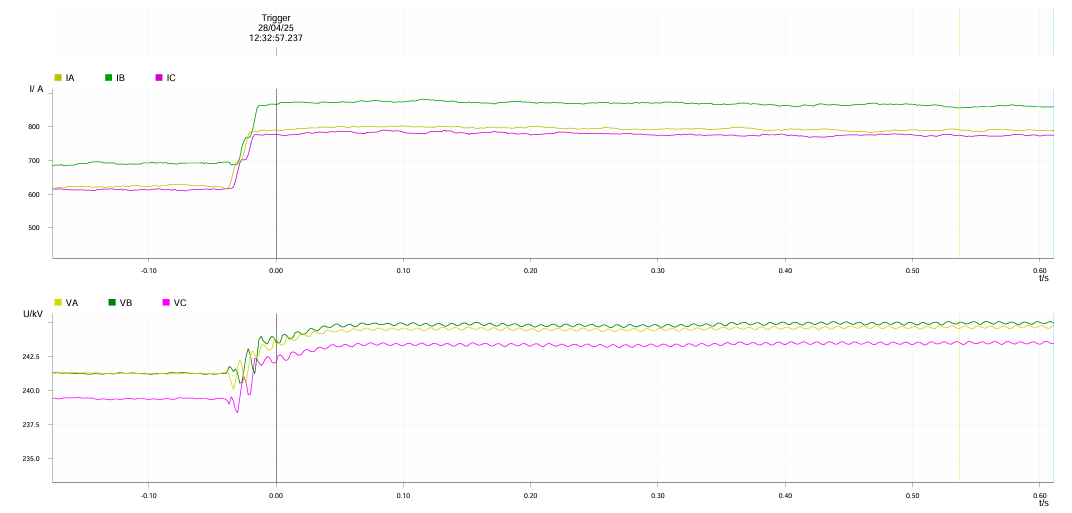
\includegraphics[width=0.9\textwidth]{figuras/disparo_raiz_oscilografia.png}
    \vspace{0.2cm}
    \caption[Registro oscilográfico del disparo raíz a las 12:32:57.]{%
    Registro oscilográfico del disparo raíz a las 12:32:57~CEST.
    Fuente: Informe de Red Eléctrica}
    \label{fig:disparo_raiz}
\end{figure}
\vspace{0.6cm}

Como se aprecia en la figura~\ref{fig:disparo_raiz}, la desconexión
eliminó instantáneamente un sumidero de 165~MVAr de reactiva
inductiva. La magnitud del impacto, según el análisis pericial, no
residió en los 355~MW de potencia activa ($P$) perdidos con la
desconexión ---una cifra manejable para el sistema---, sino en la
pérdida instantánea e irrecuperable de 165~MVAr de capacidad de
absorción de potencia reactiva ($Q$). En un sistema saturado de
reactiva capacitiva y operando con márgenes Q-V reducidos, la
desaparición de este sumidero provocó un escalón ascendente de
tensión en los nudos circundantes de la red de transporte sur. Este
rebote escalar fue, según el informe del IIT-ICAI, el detonante físico
de la inestabilidad residual de la red, iniciando la reacción en
cadena que se analiza en las secciones~\ref{sec:fase_2_tap_lag} y
\ref{sec:fase_3_cascada} \cite{icai2025}.

\section{Fase 2: el fenómeno del \textit{Tap-Lag} y el desacoplamiento de voltajes}
\label{sec:fase_2_tap_lag}

La Fase~2 del colapso, enmarcada en la ventana de los 21~s posteriores
al ``disparo raíz'', se caracteriza por la materialización de un fallo
en cascada impulsado por un fenómeno mecatrónico conocido en la
literatura como el \textit{Tap-Lag} (retardo del cambiador de tomas) o
``desacoplamiento de observabilidad''. Tras la desconexión del
transformador de Granada, la pérdida abrupta de absorción de potencia
reactiva provocó una tendencia creciente de la tensión en la red de
transporte, que reveló una divergencia entre el comportamiento de las
infraestructuras de 400~kV y las redes colectoras subyacentes
\cite{gobierno2025}.

Para comprender la mecánica de este desacoplamiento es preciso
retroceder a la Fase~1. Durante la mañana, la red había sufrido
diversas fluctuaciones y caídas de tensión originadas por las
oscilaciones de frecuencia. Para contrarrestar estas bajadas y
mantener la calidad de onda en las zonas de generación renovable, los
transformadores de interconexión 400/220~kV y 400/132~kV habían
ajustado sus \textit{Cambiadores de Tomas en Carga} (OLTC,
\textit{On-Load Tap Changer})\textsuperscript{\ref{anexo:oltc}}, subiendo las tomas para elevar el voltaje en
el lado del secundario.

\medskip

Al irrumpir la repentina sobretensión en la red de 400~kV, inducida
por el disparo de Granada, estos transformadores quedaron atrapados en
su propia inercia mecánica. Los mecanismos de motor y engranaje de los
\textit{OLTC} están ralentizados intencionadamente mediante retardos
temporales para evitar bucles de oscilación mecánica
(\textit{hunting}) ante perturbaciones efímeras. En consecuencia,
frente a un transitorio eléctrico ultrarrápido, los cambiadores
resultaron ser excesivamente lentos y no pudieron alterar su relación
de transformación a tiempo para rebajar la tensión \cite{ree2025}.

\vspace{0.6cm}
\begin{figure}[H]
    \centering
    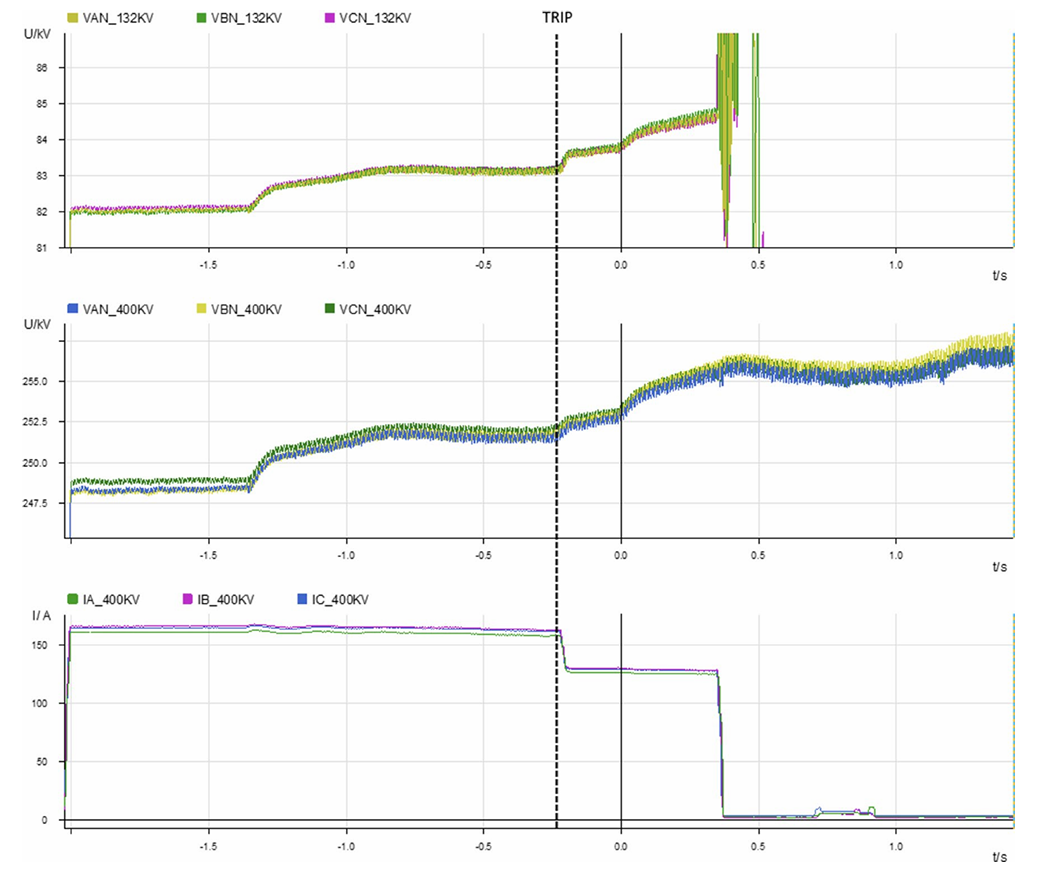
\includegraphics[width=0.70\textwidth]{figuras/tap_lag_decoupling.png} 
    \vspace{0.2cm}
    \caption[Evidencia oscilográfica del desacoplamiento de voltajes.]{%
    Evidencia oscilográfica del desacoplamiento entre el primario de
    400~kV y el secundario colector durante la Fase~2.
    Fuente: Informe Factual ENTSO-E}
    \label{fig:tap_lag_oscilografia}
\end{figure}
\vspace{0.6cm}

La figura~\ref{fig:tap_lag_oscilografia} ilustra el desacoplamiento
del fenómeno: mientras el incremento de tensión en el lado de 400~kV
se mantuvo en valores moderados, la inercia del cambiador de tomas
amplificó el transitorio en el lado colector.

Esta incapacidad mecánica creó un ``espejismo'' en la sala de control
de Red Eléctrica (REE). En las pantallas del sistema de supervisión
centralizado (\textit{Supervisory Control and Data Acquisition},
SCADA), el operador del sistema monitorizaba el primario de la red de
400~kV, observando tensiones altas pero que se mantenían
teóricamente por debajo del límite excepcional normativo de 435~kV
establecido en el Procedimiento de Operación 1.1 \cite{gobierno2025}.
Sin embargo, debido a la relación de transformación desfasada del
\textit{OLTC}, el voltaje experimentó un efecto multiplicador hacia
las redes colectoras. Aguas abajo, en las redes de 220~kV y 132~kV,
el voltaje se elevó por encima de los límites térmicos y
dieléctricos tolerables, alcanzando umbrales superiores a
1,2~\textit{p.u.}\textsuperscript{\ref{anexo:pu}} que resultaban invisibles
para el despacho nacional debido a la inobservabilidad de la red
subyacente.

Frente a esta amplificación, los inversores de las plantas solares y
eólicas se enfrentaron a voltajes inasumibles para su electrónica de
potencia. Ante el riesgo de daño en sus transistores, las
instalaciones accionaron sus sistemas internos de
\textit{Overvoltage Protection} (protección de sobretensión, función
59 ANSI) para salvaguardar la integridad de los activos.

\vspace{0.6cm}
\begin{figure}[H]
    \centering
    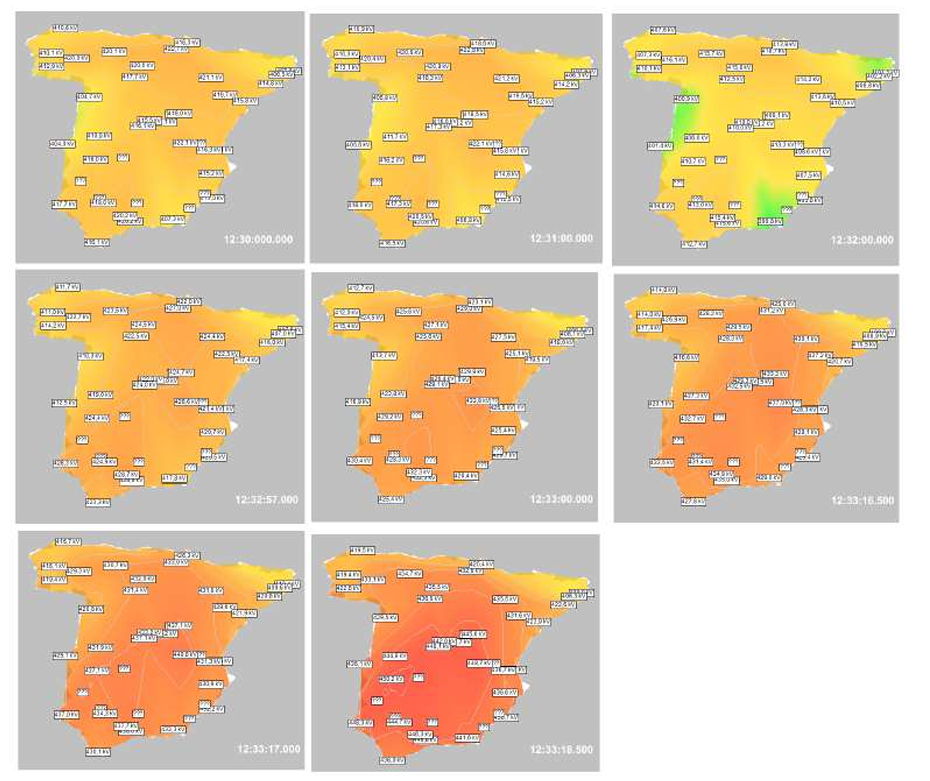
\includegraphics[width=0.90\textwidth]{figuras/heatmap_propagation.png} 
    \vspace{0.2cm}
    \caption[Propagación de las sobretensiones en la red de transporte (400 kV) durante la Fase 2.]{%
    Mapa de propagación de las sobretensiones registradas en la red de
    transporte de 400~kV durante la Fase~2 (12:32:00 -- 12:33:18~CEST).
    Fuente: Comité de Análisis del Gobierno / REE}
    \label{fig:heatmap_v}
\end{figure}
\vspace{0.6cm}

Este comportamiento fundamenta una de las mayores discrepancias
forenses del incidente, analizada en detalle en el
capítulo~\ref{cap:analisis_informes}
(p.~\pageref{cap:analisis_informes}): mientras REE tipificó estas
pérdidas como ``disparos inadecuados'' argumentando que en su red de
400~kV no existían valores de desconexión, el análisis pericial del
IIT-ICAI sostiene que las plantas actuaron de manera correcta y
adecuada a la normativa ante la sobretensión real experimentada en
sus puntos de conexión, aguas abajo del transformador con OLTC. El
fenómeno del \textit{Tap-Lag} configuró así, según dicho peritaje,
las condiciones para un bucle de retroalimentación positiva de
desconexiones en cascada.

\section{Fase 3: el camino hacia el ``Cero de Tensión''}
\label{sec:fase_3_cascada}

La Fase~3, que abarca la ventana temporal entre las 12:33:18 y las
12:33:29~CEST, escenifica el colapso total del sistema eléctrico
peninsular en apenas once segundos. Tras el inicio de los disparos por
\textit{Tap-Lag}, la red entró en un \textit{feedback loop}\textsuperscript{\ref{anexo:feedback_loop}} de inestabilidad capacitiva que ninguna intervención
humana ni automatismo de protección convencional podía detener
\cite{icai2025}.

La física de este colapso operó mediante un círculo vicioso dictado
por las ecuaciones de flujo de cargas. Al desconectarse masivamente
las plantas conectadas mediante inversores para autoprotegerse, la
red perdía instantáneamente su capacidad para absorber potencia
reactiva ($Q$). Simultáneamente, la caída de potencia activa ($P$)
reducía el flujo en las líneas de 400~kV, incrementando su inyección
capacitiva por \textit{efecto Ferranti} y empujando la tensión por
encima de los 443~kV en los nudos más estresados. Cada desconexión
elevaba la tensión, forzando nuevas desconexiones: el sistema había
entrado en un estado del que no existía salida física posible
\cite{nrel2025}.

\vspace{0.6cm}
\begin{figure}[H]
    \centering
    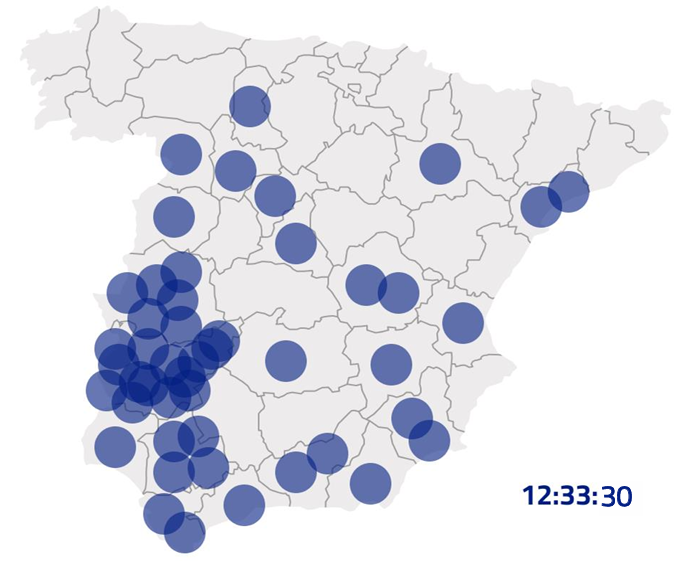
\includegraphics[width=0.65\textwidth]{figuras/cascada_desconexiones.png}
    \vspace{0.2cm}
    \caption[Propagación espacial de la pérdida de generación en cascada durante la Fase 3.]{%
    Propagación espacial de la pérdida de generación en cascada
    durante los once segundos de la Fase~3.
    Fuente: Comité de Análisis del Gobierno}
    \label{fig:mapa_cascada}
\end{figure}
\vspace{0.6cm}

La figura~\ref{fig:mapa_cascada} resume la propagación geográfica de
la cascada. Los golpes más severos se concentraron inicialmente en
Badajoz (más de 725~MW perdidos a las 12:33:16~CEST) y, un segundo
después, en las subestaciones de Segovia, Sevilla y Huelva (930~MW
adicionales a las 12:33:17~CEST). En la ventana de cinco segundos
comprendida entre las 12:33:19 y las 12:33:24~CEST, la cascada de
sobretensión desconectó más de 15~GW de generación ---cerca del
60~\% de la demanda instantánea nacional---, llevando al sistema más
allá de cualquier posibilidad de recuperación \cite{gobierno2025}.

A medida que la cascada destruía la generación remanente, la
frecuencia ($f$) comenzó a desplomarse con una tasa \textit{RoCoF}\textsuperscript{\ref{anexo:rocof}} extrema, activando los esquemas de
\textit{Deslastre Automático de Cargas por Subfrecuencia} (UFLS,
\textit{Under-Frequency Load Shedding}). Al cruzar el umbral de
49,5~Hz a las 12:33:20~CEST, se desconectaron automáticamente más
de 2.000~MW de bombeo hidráulico, seguidos de múltiples escalones
de demanda industrial a medida que la frecuencia continuaba cayendo
hasta los 48,0~Hz \cite{ree2025}.

\vspace{0.6cm}
\begin{figure}[H]
    \centering
    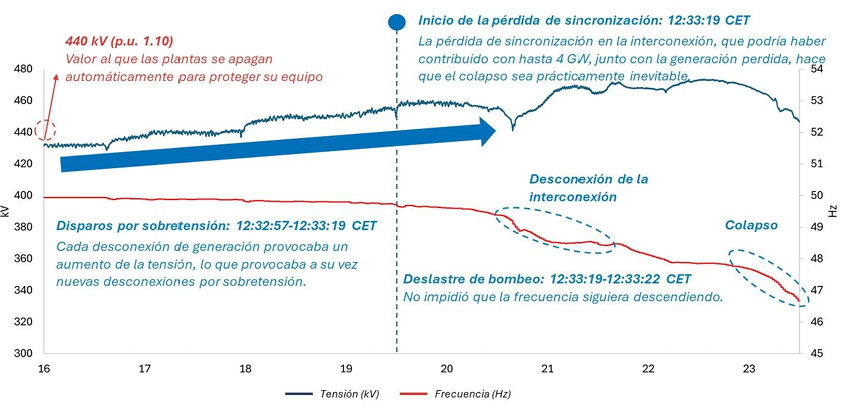
\includegraphics[width=0.95\textwidth]{figuras/tension_frecuencia_colapso.png}
    \vspace{0.2cm}
    \caption[Evolución acoplada de la tensión y la frecuencia durante el colapso.]{%
    Evolución acoplada de la tensión (kV) y la frecuencia (Hz)
    durante la Fase~3.
    Fuente: Comité de Análisis del Gobierno}
    \label{fig:v_f_acoplamiento}
\end{figure}
\vspace{0.6cm}

La figura~\ref{fig:v_f_acoplamiento} muestra la evolución acoplada de
ambas magnitudes durante la fase. Se aprecia que el incremento de
tensión por encima de 1,10~p.u. precede en el tiempo a la caída
acelerada de frecuencia, lo que apoya la interpretación del
incidente como un colapso primariamente capacitivo y no inercial.

La actuación del UFLS reveló un fenómeno electromecánico ya anticipado
en la sección~\ref{sec:eas_entsoe}: la denominada \textit{Paradoja del
UFLS}. Al cortar el consumo activo ($P$) para estabilizar la
frecuencia, el esquema de deslastre eliminó simultáneamente el
consumo de potencia reactiva ($Q$) de esa misma demanda. En una red
saturada de reactiva capacitiva, suprimir los últimos sumideros de
reactiva inductiva ---los motores y cargas industriales
desconectadas--- produjo un nuevo repunte de las sobretensiones,
reforzando el colapso que el propio UFLS pretendía frenar. Este
episodio demuestra que las lógicas de defensa del sistema diseñadas
para gestionar déficits de frecuencia pueden resultar
contraproducentes en colapsos impulsados primariamente por
inestabilidad de tensión \cite{entsoe2025}.

En los últimos instantes antes del aislamiento, el déficit masivo de
generación interna provocó una inversión violenta de los flujos en
la frontera pirenaica: las líneas AC intentaron importar desde
Francia hasta 4.609~MW de emergencia. Sin embargo, y de forma
simultánea, el enlace HVDC INELFE-1 ---fijado en modo de potencia
constante (PMODE1) desde las 12:08~CEST, como se describió en la
sección~\ref{sec:interconexiones}--- continuaba extrayendo
1.000~MW del sistema ibérico, reduciendo en un 22~\% la capacidad
de soporte neto desde Francia. El tránsito resultante se volvió
angular y térmicamente insostenible para el corredor
transfronterizo \cite{icai2025}.

\vspace{0.6cm}
\begin{figure}[H]
    \centering
    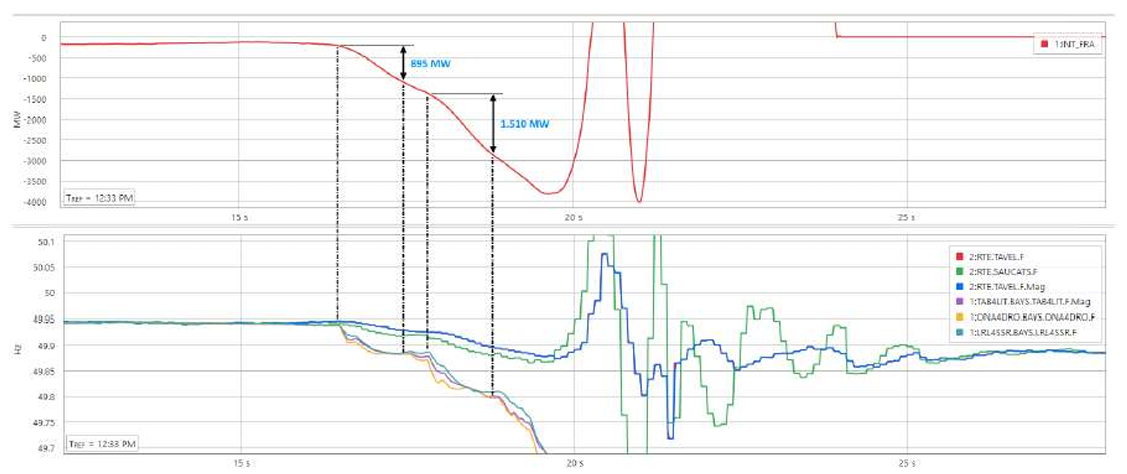
\includegraphics[width=0.85\textwidth]{figuras/interconexion_francia_colapso.png}
    \vspace{0.2cm}
    \caption[Pérdida de sincronismo y aislamiento de la península ibérica.]{%
    Intercambio con Francia y evolución de la frecuencia durante la
    Fase~3.
    Fuente: Comité de Análisis del Gobierno / REE}
    \label{fig:interconexion_francia}
\end{figure}
\vspace{0.6cm}

La figura~\ref{fig:interconexion_francia} recoge la inversión de los
flujos en la frontera pirenaica durante la Fase~3, con la
importación de emergencia de hasta 4.609~MW por las líneas AC, la
extracción simultánea por el HVDC en modo de potencia constante y la
apertura de las líneas AC por pérdida de sincronismo a las
12:33:21~CEST.

A las 12:33:21~CEST, las protecciones de pérdida de sincronismo
abrieron los enlaces de corriente alterna para evitar el contagio
al sistema europeo continental, aislando la península ibérica.
Convertida en una isla eléctrica sin capacidad de autosostén
tensional, las escasas máquinas síncronas remanentes se
desconectaron en cascada. El ``Cero de Tensión'' definitivo se
confirmó a las 12:33:29.741~CEST con el disparo del último grupo
generador, cerrando el incidente sistémico más severo documentado
en la historia del sistema eléctrico europeo continental
\cite{gobierno2025}.